\documentclass[11pt]{article}
\usepackage[T1]{fontenc}
\usepackage{lmodern}
\usepackage[margin=1in]{geometry}
\usepackage{amsmath,amssymb}
\usepackage{microtype}
\usepackage{graphicx}
\usepackage{subcaption}
\usepackage{fancyhdr}

% ---- fill in before submitting ----
\newcommand{\studentname}{Harshit Gupta}
\newcommand{\studentid}{Student ID}
% -----------------------------------

\pagestyle{fancy}
\fancyhf{}
\fancyhead[L]{\small CSE 242 \,|\, Assignment 4}
\fancyhead[R]{\small \studentname}
\fancyfoot[C]{\small \thepage}
\setlength{\parindent}{0pt}
\setlength{\parskip}{0.55em}
\graphicspath{{../results/kmeans/}{../results/noisy_labels/}}

\newcommand{\N}{\mathcal{N}}

\begin{document}
\begin{center}
  {\LARGE\bfseries Assignment 4: Clustering and Learning with Noisy Data}\\[0.4em]
  \studentname \,|\, \studentid
\end{center}

\section*{Part 1: EM for Gaussian mixture models}

Each observation $x_i$ has a hidden label $z_i\in\{1,\dots,K\}$. The mixture model
assumes $P(z_i=k)=\pi_k$ and $p(x_i\mid z_i=k)=\N(x_i;\mu_k,\Sigma_k)$, with the pairs
$(x_i,z_i)$ independent across $i$.

\subsection*{1.1 E-step}

\textbf{Bayes' rule.}
\[
r_{ik}=P(z_i=k\mid x_i,\theta)=\frac{p(x_i\mid z_i=k)\,P(z_i=k)}{p(x_i)}.
\]
\textbf{Mixture assumptions.} The numerator is $\N(x_i;\mu_k,\Sigma_k)\,\pi_k$. The
denominator sums the same product over every value the label can take, by the law of
total probability: $p(x_i)=\sum_{j}\pi_j\,\N(x_i;\mu_j,\Sigma_j)$. Therefore
\[
r_{ik}=\frac{\pi_k\,\N(x_i;\mu_k,\Sigma_k)}{\sum_{j=1}^{K}\pi_j\,\N(x_i;\mu_j,\Sigma_j)}.
\]

\subsection*{1.2 M-step}

\textbf{Independence of observations.} With the labels known, the log likelihood is a sum
over $i$: $\log p(X,Z;\theta)=\sum_i\sum_k\mathbf{1}[z_i=k]\,
\bigl(\log\pi_k+\log\N(x_i;\mu_k,\Sigma_k)\bigr)$.

\textbf{Expectation.} This is linear in the indicators, and
$\mathbb{E}\bigl[\mathbf{1}[z_i=k]\mid x_i\bigr]=r_{ik}$, so
\[
Q(\theta)=\sum_{i=1}^{n}\sum_{k=1}^{K}r_{ik}\,\bigl(\log\pi_k+\log\N(x_i;\mu_k,\Sigma_k)\bigr).
\]
The $r_{ik}$ are fixed during the M-step. Let $N_k=\sum_i r_{ik}$.

\textbf{Update for $\mu_k$.} Only
$-\tfrac12\sum_i r_{ik}\,(x_i-\mu_k)^{\!\top}\Sigma_k^{-1}(x_i-\mu_k)$ contains $\mu_k$.

\emph{Derivative of a sum:}
$\nabla_{\mu_k}Q=\Sigma_k^{-1}\sum_i r_{ik}\,(x_i-\mu_k)$.

\emph{First-order optimality condition:} set the gradient to zero and multiply by
$\Sigma_k$, giving $\sum_i r_{ik}x_i=N_k\,\mu_k$, so
\[
\mu_k=\frac{1}{N_k}\sum_{i=1}^{n}r_{ik}\,x_i .
\]

\textbf{Update for $\pi_k$.} Only $\sum_k N_k\log\pi_k$ contains $\pi$, and the weights
must satisfy $\sum_k\pi_k=1$.

\emph{Lagrange multiplier:}
$\mathcal{L}=\sum_k N_k\log\pi_k+\lambda\bigl(1-\sum_k\pi_k\bigr)$.

\emph{First-order optimality condition:} $N_k/\pi_k-\lambda=0$, so $\pi_k=N_k/\lambda$.

\emph{Constraint:} summing over $k$ gives $\lambda=\sum_k N_k=\sum_i\sum_k r_{ik}=n$, so
\[
\pi_k=\frac{N_k}{n}.
\]

\section*{Part 2: Exploring structure with K-means}

\subsection*{2.1 Dataset and question}

\textbf{Dataset.} The Dry Bean Dataset of Koklu and Ozkan (2020), from the UCI Machine
Learning Repository. It has 13{,}611 bean grains from seven registered varieties, each
measured from a photograph. One observation is one bean.

\textbf{Features.} All 16 numerical shape measurements, which cover size (area, perimeter,
axis lengths) and form (aspect ratio, roundness, compactness, four shape factors).

\textbf{Preprocessing.} I removed 68 exact duplicate rows, leaving 13{,}543 beans, and
standardized every feature to mean 0 and standard deviation 1. The raw columns run from
0.0006 to 254{,}616, so without scaling the area columns alone would decide every
distance. The variety labels play no part in fitting.

\textbf{Why cluster, and the question.} Breeders define the varieties, not these 16
measurements, so the measurements may not split into seven groups. \emph{Do the seven
varieties appear as separate groups in shape space, and if not, which ones can shape
alone not tell apart?}

\subsection*{2.2 K-means from scratch}

The implementation is in \texttt{kmeans\_clustering.py} and uses NumPy only.

\textbf{Initialization.} k-means++: the first centroid is a random data row, and each
later one is a row drawn with probability proportional to its squared distance from the
nearest centroid already chosen.

\textbf{Assignment and update.} Each point goes to the closest centroid by squared
Euclidean distance, with ties going to the lowest centroid index. Each centroid then
moves to the mean of its points.

\textbf{Stopping.} The loop stops when no assignment changes or no centroid moves more
than $10^{-6}$, and after 100 iterations at the latest.

\textbf{Empty clusters.} A cluster with no points keeps its previous centroid. This never
happened in the runs below.

\subsection*{2.3 Choosing $K$}

I ran $K=2$ to $10$ with \texttt{-{}-seed 0}, each from 10 random starts, keeping the run
with the lowest within-cluster sum of squares (WCSS). Stability is the mean adjusted Rand
index between every pair of the 10 starts, where 1 means all starts found the same
partition.

\begin{center}
\begin{tabular}{lrrrrrrrrr}
\hline
$K$ & 2 & 3 & 4 & \textbf{5} & 6 & 7 & 8 & 9 & 10\\
\hline
WCSS (thousands) & 129.2 & 94.3 & 76.0 & \textbf{61.6} & 54.9 & 48.7 & 45.1 & 41.9 & 39.7\\
Mean silhouette & 0.397 & 0.405 & 0.342 & \textbf{0.357} & 0.360 & 0.309 & 0.303 & 0.303 & 0.271\\
Stability & 1.000 & 0.820 & 0.721 & \textbf{0.922} & 0.799 & 0.876 & 0.697 & 0.661 & 0.681\\
\hline
\end{tabular}
\end{center}

\textbf{I chose $K=5$.} Each added cluster up to $K=5$ removes at least 19\% of the WCSS, and each one after removes 11\% or less, so the elbow is at 5. Apart from
$K=2$, it is also the most stable solution. The silhouette is higher at $K=2$ and $K=3$,
but $K=3$ only separates the largest variety, the other large beans and the small
beans, which is too coarse for the question. Among $K\ge4$ the silhouette is highest at 5
and 6.

\subsection*{2.4 Visualization and analysis}

\begin{figure}[t]
  \centering
  \begin{subfigure}{0.38\textwidth}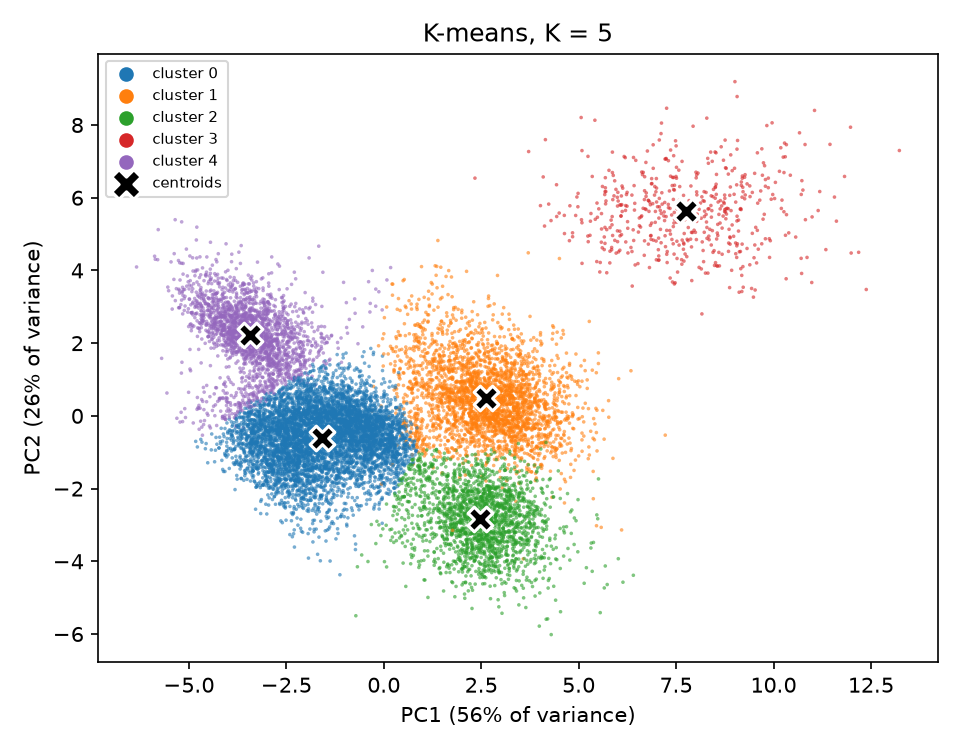
\includegraphics[width=\linewidth]{pca_clusters_k5.png}
    \caption{K-means clusters, $K=5$}\end{subfigure}\hspace{0.04\textwidth}
  \begin{subfigure}{0.38\textwidth}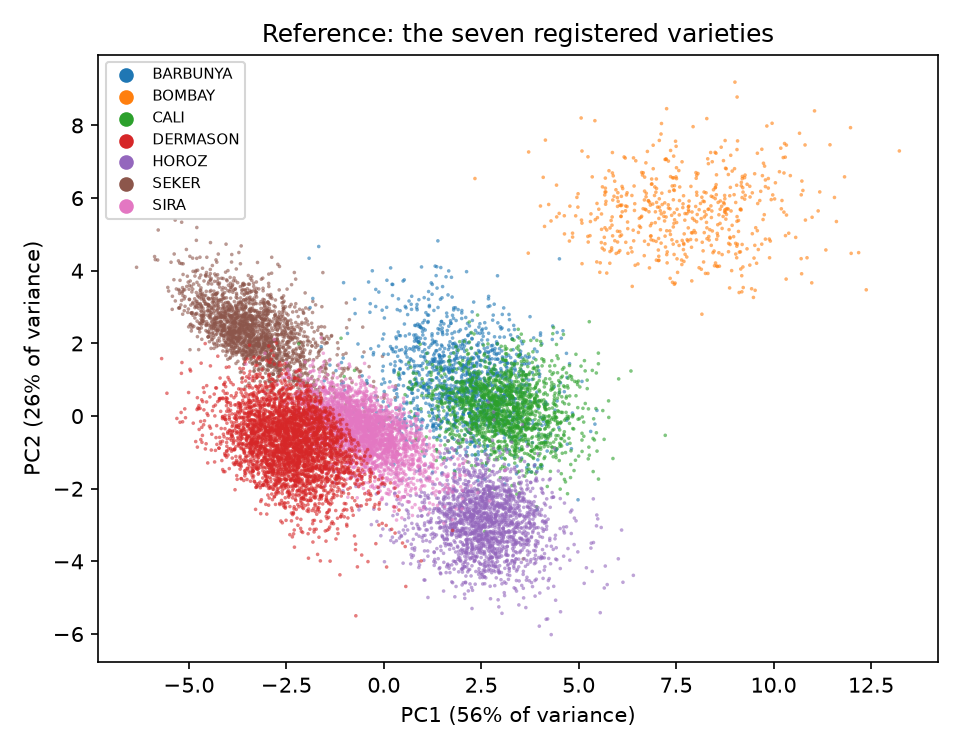
\includegraphics[width=\linewidth]{pca_varieties.png}
    \caption{True varieties}\end{subfigure}
  \caption{The beans on their first two principal components. PCA is used for plotting
  only. K-means ran on all 16 features.}
  \label{fig:pca}
\end{figure}

\textbf{What distinguishes the clusters.} Size and elongation. In standard deviations from
the mean, cluster 3 has area $+4.1$, cluster 1 has area $+0.7$ and cluster 0 has area
$-0.5$. Cluster 2 is elongated, with aspect ratio $+1.8$, and cluster 4 is round, with
aspect ratio $-1.4$.

\textbf{Does it answer the question?} Partly. Reading the labels after clustering, Bombay,
Seker and Horoz each get their own cluster, holding 521 of 522, 93\% and 96\% of their
beans. Cluster 0 holds 92\% of Dermason together with 90\% of Sira, and cluster 1 holds
93\% of Barbunya together with 97\% of Cali. Shape finds five groups, and those two pairs
are the varieties it cannot tell apart.

\textbf{Ambiguous points.} For 11.6\% of the beans the nearest centroid is at least 0.8
times as far away as the second-nearest, so the hard assignment is close to arbitrary.
These beans lie between clusters 0, 1 and 2, where one variety shades into the next
without a gap.

\textbf{Limitation.} K-means puts a straight boundary halfway between two centroids,
which suits round groups of similar spread. The varieties in Figure~\ref{fig:pca}(b) are
tilted ellipses of different sizes that overlap, so no such boundary separates Dermason
from Sira.

\section*{Part 3: Classification with noisy labels}

\subsection*{3.1 Baseline and evaluation design}

\textbf{Task.} Predict the variety of a bean, one of seven classes, from the 16 features
of Part 2. The code is in \texttt{noisy\_classification.py}, run with
\texttt{-{}-seed 0 -{}-trials 10}.

\textbf{Split.} One stratified split with seed 0: 8{,}126 training, 2{,}710 validation and
2{,}707 test beans, which is 60/20/20. I standardized the features with the training
mean and standard deviation. The test labels are never corrupted.

\textbf{Metrics.} Accuracy and macro-F1. The classes are unbalanced, from 522 Bombay
beans to 3{,}546 Dermason, and macro-F1 weights every variety equally.

\textbf{Classifier.} An RBF-kernel SVM. I tuned $C\in\{0.1,1,10,100\}$ and
$\gamma\in\{0.01,0.03,0.1,0.3\}$ on validation accuracy, which selected $C=1$ and
$\gamma=0.1$. Every experiment below uses these values.

\textbf{Clean baseline.} Test accuracy 0.9313, macro-F1 0.9409.

\subsection*{3.2 Label noise}

Each training label is resampled once, from a distribution that depends only on its true
class. I used two noise types at rates $\rho=0.20$ and $\rho=0.40$.

\textbf{Uniform.} A label is kept with probability $1-\rho$. Otherwise it becomes one of
the six other varieties, each with probability $\rho/6$.

\textbf{Look-alike, which is class-dependent and asymmetric.} A label is kept with
probability $1-\rho$. Otherwise it becomes the variety whose training centroid is nearest
to its own: Barbunya $\to$ Cali, Bombay $\to$ Cali, Cali $\to$ Barbunya, Dermason $\to$
Sira, Horoz $\to$ Cali, Seker $\to$ Dermason, Sira $\to$ Dermason. Bombay labels can
become Cali, but no Cali label becomes Bombay.

\textbf{Why this is a reasonable stress test.} People sorting beans confuse the varieties
that look alike, not random pairs, and these are the pairs Part 2 could not separate.
Uniform noise is the reference case with no structure. The 40\% rate is close to the
50\% at which the wrong label would become the more common one. The table in 3.4 compares
the SVM trained on each noisy set with the clean baseline.

\subsection*{3.3 Repair strategy: nearest-neighbour vote with a threshold}

The repair runs once on the training labels, before the SVM of 3.1 is trained. For each
training bean $i$ with noisy label $\tilde y_i$:
\vspace{-0.6em}
\begin{enumerate}\setlength{\itemsep}{0pt}\setlength{\parskip}{0pt}
\item Find its $k$ nearest other training beans by Euclidean distance on the
  standardized features.
\item Let $s_i(c)$ be the share of those neighbours whose noisy label is $c$, and
  $c^\ast$ the class with the largest share.
\item Replace $\tilde y_i$ by $c^\ast$ only if $c^\ast\neq\tilde y_i$,
  $s_i(c^\ast)\ge\tau$ and $s_i(c^\ast)>s_i(\tilde y_i)$.
\end{enumerate}
\vspace{-0.6em}
Every vote uses the original noisy labels, so row order does not matter.

\textbf{Reasoning.} A label that most similar beans contradict is probably wrong. The
threshold $\tau$ protects borderline beans, which a narrow majority can outvote even when
their label is correct. A larger $k$ gives a more reliable vote under heavy noise but
reaches across class boundaries.

\textbf{Choosing $k$ and $\tau$.} For each noise setting I tried $k\in\{5,15,45,135\}$
and $\tau\in\{0.5,0.6,0.7\}$ on a separate noise draw and kept the pair with the best
validation accuracy. This assumes the validation labels are trusted. The repair itself
sees only training features and noisy training labels.

\subsection*{3.4 Controlled comparison}

All conditions share the SVM, the clean test set and, within a trial, the corrupted
labels. Values are the mean and sample standard deviation over 10 trials.

\begin{center}
\begin{tabular}{llccc}
\hline
Noise & Training labels & Wrong labels & Test accuracy & Test macro-F1\\
\hline
None & Clean & 0\% & 0.9313 & 0.9409\\
\hline
Uniform 20\% & Noisy & 19.9\% & $0.9310\pm0.0013$ & $0.9407\pm0.0012$\\
 & Repaired, $k=45$, $\tau=0.7$ & 6.9\% & $0.9301\pm0.0012$ & $0.9400\pm0.0014$\\
\hline
Uniform 40\% & Noisy & 39.8\% & $0.9287\pm0.0013$ & $0.9383\pm0.0013$\\
 & Repaired, $k=15$, $\tau=0.7$ & 33.5\% & $0.9285\pm0.0017$ & $0.9383\pm0.0018$\\
\hline
Look-alike 20\% & Noisy & 20.1\% & $0.9280\pm0.0018$ & $0.9388\pm0.0015$\\
 & Repaired, $k=5$, $\tau=0.5$ & 13.5\% & $0.9289\pm0.0017$ & $0.9397\pm0.0014$\\
\hline
Look-alike 40\% & Noisy & 39.9\% & $0.9050\pm0.0097$ & $0.9137\pm0.0104$\\
 & Repaired, $k=45$, $\tau=0.6$ & 24.1\% & $0.9125\pm0.0065$ & $0.9230\pm0.0066$\\
\hline
\end{tabular}
\end{center}

The method does not help consistently. It helps in one regime, look-alike noise at 40\%.
There the noise costs 2.63 points of accuracy, and repair wins back $0.0075\pm0.0055$ and
beats the noisy classifier in 9 of 10 trials. At 20\% look-alike noise the gain of $0.0009\pm0.0023$
is smaller than the variation between trials. Under uniform noise there is no gain,
$-0.0009\pm0.0018$ and $-0.0001\pm0.0013$, because uniform noise costs at most 0.26 points to begin with.

\subsection*{3.5 Reflection}

The strategy helped only when the noise was heavy and structured, which is the one case
where the noise had moved the SVM's boundary. Under uniform noise there was nothing to
fix, and repair was neutral or slightly harmful. It has a cost even without noise:
applied to the clean labels, it changed 3.2\% of them to a wrong variety and accuracy
fell from 0.9313 to 0.9306. It also depends on trusted validation labels. When I chose
$k$ and $\tau$ against validation labels carrying the same noise, with
\texttt{-{}-selection noisy}, the gain at 40\% look-alike noise fell to
$0.0001\pm0.0009$.

The method assumes that beans close in Euclidean distance share a variety. That fails
where Dermason overlaps Sira and Barbunya overlaps Cali, which is where correct labels
matter most. It also assumes the true variety still holds the most labels in every
neighbourhood, so the noise must stay below 50\% and must not concentrate on borderline
beans. Before changing labels automatically on real data I would want an expert to check
a random sample of labels, to learn how much noise there is and whether it is structured,
and a sample of the proposed changes, to learn how often the repair is right. I would
also want a trusted validation set showing that the classifier improves. Without that
evidence I would use the vote to flag labels for review, not to overwrite them.

\section*{Acknowledgment of outside help}
\textbf{Dataset and software.} Dry Bean Dataset, M.~Koklu and I.~A.~Ozkan (2020), from
the UCI Machine Learning Repository. The code uses NumPy, scikit-learn, Matplotlib and
the function names of the optional starter file.

\textbf{Generative AI.} I used a generative AI assistant (Claude, Anthropic, via
Claude Code) on this assignment. It helped with the derivations, the choice of dataset,
the code, the experiments, the figures and the drafting of this report. The full
conversation log is submitted with this assignment, as the course AI policy requires. I
have checked the results by rerunning the commands in \texttt{README.md}.


\end{document}
